\chapter{A Private Cloud for MapReduce Applications}\label{cap:solucion}
\noindent This chapter introduces a novel solution combining the virtual infrastructure managed with OpenStack and the Hadoop implementation of MapReduce to conform a powerful computational tandem. \emph{qosh}, as this project has been called, will be described along this section moving from architecture to implementation.

\section{Architecture}\label{sec:diseno}
\noindent Figure \ref{fig:arquitecturaglobal} shows a high level portrait of qosh execution environment. The component that acts as interface between system and user is displayed on the right end. It abstracts the inherent difficulty in configuring the job execution context and in deploying the virtual cluster. Furthermore, qosh will keep track of submitted jobs, MapReduce \texttt{jar} files, input data and output results, with no need to walk the HDFS to search for data.

\begin{figure}[tbp]
\begin{center}
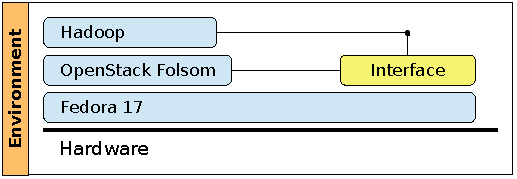
\includegraphics[width=0.65\textwidth]{imagenes/021.pdf}
 \caption{Global Architecture}
\label{fig:arquitecturaglobal}
\end{center}
\end{figure}

Se determina que el hardware soporte de la primera versi\'on del proyecto sea un computador personal para agilizar el desarrollo. Como muestra la figura \ref{fig:arquitecturaglobal}, sobre el hardware se instala el sistema operativo (Fedora 17) y sobre \'el OpenStack Folsom. No obstante, ha de tenerse en cuenta que ser\'ia \'optimo permitir que la interfaz pudiese gestionar ejecuciones MapReduce en un cloud remoto. As\'i estar\'iamos flexibilizando al m\'aximo el aprovisionamiento de infraestructura virtual que otorgan los cloud, sin estar limitados por las capacidades que pudiesen presentar nuestras instalaciones locales. En esta fase de dise\~no de alto nivel no nos centraremos en elaborar esa idea, pero s\'i es interesante que la tengamos presente. \newline

La figura \ref{fig:arquitecturadetalle} representa la ampliaci\'on de los detalles de dise\~no de alto nivel expuestos en la figura \ref{fig:arquitecturaglobal}. La m\'aquina virtual contiene la instalaci\'on de Hadoop 1.0.4. Es gestionada por OpenStack y se ejecuta a cargo de KVM, el hipervisor seleccionado. Como se ve en la figura, se ha elegido el propio DFS de Hadoop (HDFS) para almacenar los datos de entrada y de salida del cl\'uster mientras no se hayan transferido al controlador del cloud. Recordemos que estamos hablando del almacenamiento vol\'atil de los cloud, es decir, toda informaci\'on que no haya sido extra\'ida de las m\'aquinas virtuales se perder\'a al concluir su ejecuci\'on. De modo que es nuestra tarea manejar la informaci\'on de salida; se ha decidido que sea almacenada en el nodo que sirva las p\'aginas web ---el nodo que ejecute Django.\newline

\begin{figure}[tbp]
\begin{center}
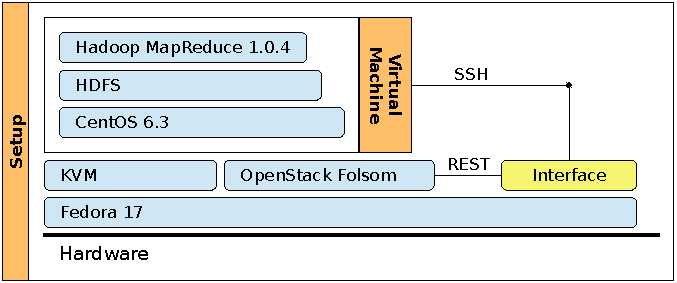
\includegraphics[width=0.85\textwidth]{imagenes/022.pdf}
 \caption{Arquitectura global en detalle}
\label{fig:arquitecturadetalle}
\end{center}
\end{figure}

La figura \ref{fig:arquitecturainterfaz} contiene la visi\'on de alto nivel de los distintos m\'odulos participantes en la orquestaci\'on de las ejecuciones.

\begin{figure}[bp]
\begin{center}
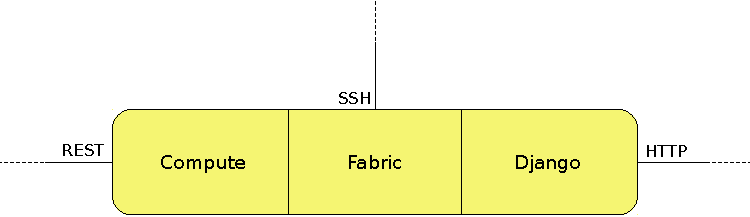
\includegraphics[width=0.8\textwidth]{imagenes/023.pdf}
 \caption{Composici\'on modular de la interfaz}
\label{fig:arquitecturainterfaz}
\end{center}
\end{figure}

\begin{description}
 \item[Compute:] es el cliente de acceso que se encarga de concretar toda interacci\'on con el API REST de OpenStack, desacoplando el resto del proyecto del cloud concreto que genere la infraestructura virtual.
 \item[Django:] es un framework escrito en Python para crear y mantener sitios web completos.
 \item[Fabric:] es una librer\'ia Python (2.5+) y herramienta CLI para facilitar y mejorar el uso de SSH para el despliegue de aplicaciones o la ejecuci\'on de tareas de administraci\'on de sistemas.
\end{description}


\subsection{Diagramas de dise\~no}\label{subsec:diagramasaltonivel}
\noindent A continuaci\'on se muestran los diagramas que completan la secci\'on de comentarios del dise\~no de alto nivel del proyecto.


\subsubsection{Componentes de Django}\label{subsubsec:componentesdjango}
\noindent La figura \ref{fig:instalaciondjango} muestra los m\'odulos adyacentes a Django que se han seleccionado para apoyar su ejecuci\'on.

\begin{figure}[bp]
\begin{center}
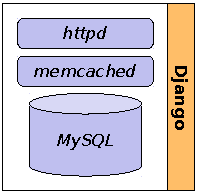
\includegraphics[width=0.23\textwidth]{imagenes/024.pdf}
 \caption{Instalaci\'on concreta de Django}
\label{fig:instalaciondjango}
\end{center}
\end{figure}

\begin{description}
 \item[Apache httpd:] conocido servidor web seguro, eficiente y extensible.
 \item[memcached:] m\'odulo de \emph{caching} utilizado extensamente en distintos \'ambitos. Django se vale de \'el para acelerar la carga de p\'aginas y sesiones de usuario.
 \item[MySQL:] una de las implementaciones de base de datos relacional m\'as utilizadas. Se acopla a Django para que la informaci\'on de los usuarios registrados en el cloud, sus sesiones en ejecuci\'on y los datos relacionados con todas las peticiones de procesado de trabajos MapReduce sea persistente.
\end{description}


\subsubsection{Diagrama de Casos de Uso}\label{subsubsec:casosuso}
\noindent La figura \ref{fig:casosuso} contiene el conjunto de casos de uso del proyecto. Refleja los cinco agentes fundamentales que interact\'uan en el sistema. Aqu\'i se pone de manifiesto la necesidad de tener una sesi\'on iniciada contra el servidor de la interfaz para interactuar con ella.

\begin{figure}[tbp]
\begin{center}
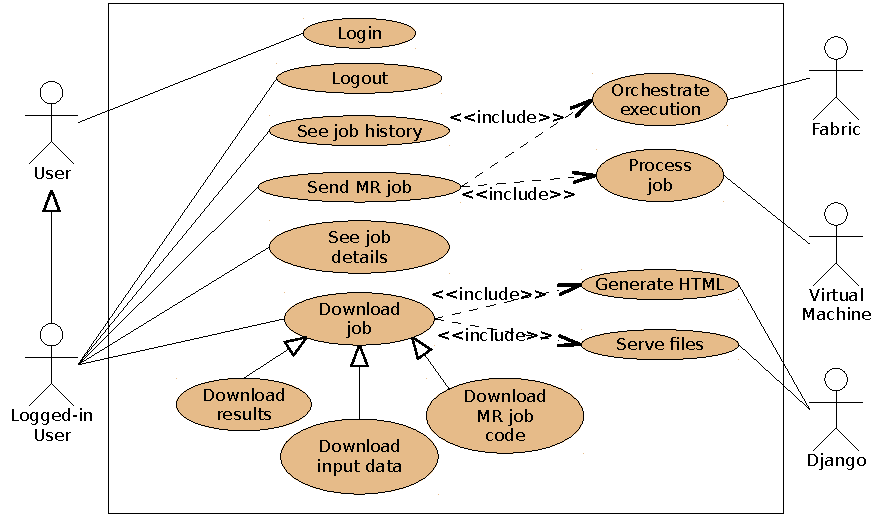
\includegraphics[width=0.99\textwidth]{imagenes/025.pdf}
 \caption{Diagrama de Casos de Uso}
\label{fig:casosuso}
\end{center}
\end{figure}



\subsubsection{Diagrama de M\'aquina de Estados}\label{subsubsec:navegacion}
\noindent La figura \ref{fig:navegacion} representa el flujo de navegaci\'on por la interfaz web mediante un diagrama de M\'aquina de Estados. Analicemos, fij\'andonos en la figura, una interacci\'on del usuario con el sistema.\newline

Inicialmente, al usuario se le presenta la p\'agina de \emph{Login} para que pueda conectarse. Si las credenciales que aporta son correctas, y lo ser\'an si el usuario est\'a dado de alta en OpenStack ---el login se delega en el sistema de autenticaci\'on de OpenStack---, se le presenta la p\'agina \emph{Principal}. Desde ah\'i podr\'a \emph{Configurar trabajo} o acceder al \emph{Historial} de trabajos en\-via\-dos. Sin duda, la parte gruesa del proceso reside en la transici\'on \emph{Enviar trabajo} que pondr\'a en marcha la ejecuci\'on del trabajo definido.

\begin{figure}[tbp]
\begin{center}
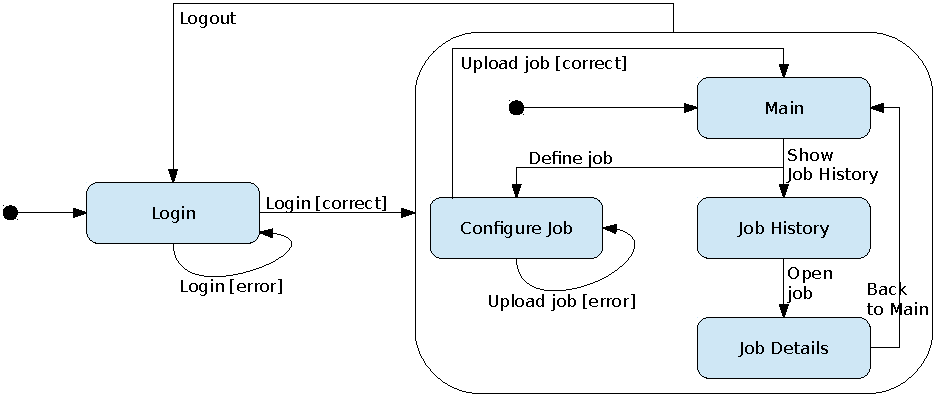
\includegraphics[width=0.99\textwidth]{imagenes/026.pdf}
 \caption{M\'aquina de Estados de la interfaz web}
\label{fig:navegacion}
\end{center}
\end{figure}


\subsubsection{Diagrama de Clases --- M\'odulo Compute}\label{subsubsec:diagramaclasescompute}
\noindent La figura \ref{fig:diagramaclasescompute1} muestra un peque\~no Diagrama de Clases que describe las relaciones del cliente de acceso al API REST con algunos m\'odulos de Fabric y Python.

\begin{description}
 \item[json:] \emph{parsea} y maneja datos estructurados en formato JSON. El API REST de OpenStack entiende tanto XML como JSON.
 \item[Exception:] clase Python que representa una excepci\'on gen\'erica.
 \item[ServiceError:] extensi\'on de \texttt{Exception}. Se utiliza como contenedor de los errores que pudiesen aparecer al interactuar con el servicio REST. Est\'a compuesto por el c\'odigo y la descripci\'on del error HTTP que se produzca.
 \item[Environment:] recoge las variables globales de configuraci\'on de la interfaz.
 \item[httplib:] es el paquete Python que contiene las funciones y clases necesarias para establecer comunicaciones HTTP. Se usa en este proyecto para consumir el servicio REST.
\end{description}

\begin{figure}[tbp]
\begin{center}
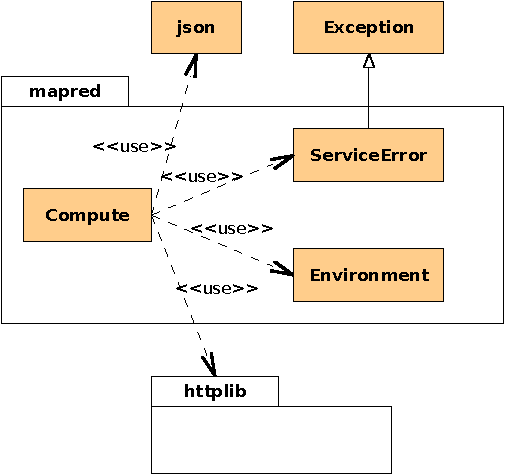
\includegraphics[width=0.5\textwidth]{imagenes/027.pdf}
 \caption{Diagrama de Clases del cliente de acceso REST (I)}
\label{fig:diagramaclasescompute1}
\end{center}
\end{figure}


\section{Implementaci\'on}\label{sec:implementacion}
\noindent Los tres m\'odulos que componen la interfaz se han escrito en Python. Las pruebas de la primera versi\'on corren sobre las versiones 1.4.3 de Fabric, 1.4.2 de Django y 2.7.3 de Python. La configuraci\'on dentro de la m\'aquina virtual, para permitir su acceso desde el cloud, se realiza con tres scripts, escritos en \texttt{bash-script}, que se activan en tres momentos diferentes del ciclo de vida del servidor virtual: antes de configurar la red, despu\'es de haber arrancado con \'exito y antes de destruirse.


\subsection{M\'aquina virtual}\label{subsec:maquinavirtual}
\noindent Una parte importante del proyecto ha sido la construcci\'on de la m\'aquina virtual que contiene la instalaci\'on de Hadoop 1.0.4 y el JRE 1.7 de Oracle. Su configuraci\'on y puesta a punto no result\'o un proceso muy complejo, pero s\'i lo suficientemente interesante y largo, por ser reutilizable para cualquier m\'aquina virtual que se pretenda preparar para correr en un cloud, como para elaborar una lista con todos los pasos seguidos. El entorno de instalaci\'on es el citado MacBook 6,1 bajo un Fedora 17 actualizado.
\begin{itemize}
    \item Se a\~nadi\'o con \texttt{yum} el \emph{Virtual Machine Manager} (\texttt{virt-manager}) y sus librer\'ias dependientes, entre las que destacamos: la librer\'ia de vir\-tua\-li\-za\-ci\'on (\texttt{libvirt}), el m\'odulo del kernel para el hypervisor (KVM) y un \emph{wrapper} de ese m\'odulo para gestionar su uso (QEMU).
 \item Utilizando el Virtual Machine Manager se configur\'o una m\'aquina virtual con 1 GB de RAM, 4 GB de disco en formato \emph{QCOW2} y tanto APIC como ACPI.
 \item Se prosigui\'o con la instalaci\'on en red de la \'ultima versi\'on estable de CentOS (la 6.3), eligiendo \emph{Basic Server} como conjunto de paquetes instalados por defecto; en una sola partici\'on ext4 y sin LVM.
 \item Al reiniciar, se pidi\'o a yum que actualizase todos los paquetes del sistema.
 \item Se descargaron desde las webs oficiales las versiones comentadas del JRE y Hadoop y se instalaron con \texttt{rpm}.
 \item Se cre\'o el usuario \emph{hduser} con grupo principal \emph{hadoop} y se retocaron los permisos de los ficheros relacionados con Hadoop ---ficheros de con\-fi\-gu\-ra\-ci\'on y scripts.
 \item Se configur\'o \texttt{sshd} para impedir la conexi\'on como \emph{root} y el acceso utilizando nombre de usuario y contrase\~na como credenciales; s\'olo se permite establecer t\'uneles SSH usando la parte privada de la clave que inyecta OpenStack en la m\'aquina virtual en cada arranque.
 \item Se escribieron tres scripts (\texttt{/etc/init.d/cloud-*}) para personalizar el comportamiento de la m\'aquina virtual, como escribir en su lugar (\texttt{/home/hduser/.ssh/authorized\_keys}) la clave p\'ublica de acceso SSH inyectada por el cloud.
 \item Se eliminaron, con \texttt{yum groups}, servicios no utilizados, como el \emph{X-server}.
 \item Se compact\'o la imagen QCOW2 creando un fichero indeterminadamente grande, con \texttt{dd}, y comprimiendo, desde el anfitri\'on, con \texttt{qemu-img}.
 \item Con \texttt{qemu-nbd} se mont\'o la imagen de la m\'aquina virtual como un dispositivo de bloque en red y con \texttt{fdisk} se observaron el tama\~no del bloque y el bloque inicial de la partici\'on que contiene la instalaci\'on de Hadoop, para calcular su desplazamiento con respecto al inicio del disco virtual.
 \item Finalmente, de nuevo con \texttt{qemu-nbd} se mont\'o la imagen con el des\-pla\-za\-mien\-to calculado, para extraer la \'unica partici\'on (la ra\'iz) del disco virtual contenido en la imagen. Asimismo, se copiaron al anfitri\'on tanto el kernel como la \emph{initram} de la instalaci\'on de CentOS.
\end{itemize}



\subsection{Diagramas de implementaci\'on}\label{subsec:diagramasimpl}
\noindent Acto seguido se exponen aquellos diagramas que describen el proyecto desde un punto m\'as cercano a su implementaci\'on.


\subsubsection{Diagrama de Clases --- M\'odulo Compute}\label{subsubsec:implementacioncompute}
\noindent La figura \ref{fig:diagramaclasescompute2} expande el detalle del m\'odulo \texttt{Compute} de la figura \ref{fig:diagramaclasescompute1}. El comportamiento de las funciones se deduce f\'acilmente de las firmas de la figura. Si cabe, destacar que la nomenclatura utilizada para describir algunos tipos de funciones ---un tipo diccionario y un tipo lista, recuerda a la sintaxis de Python que declara esos tipos.

\begin{figure}[tbp]
\begin{center}
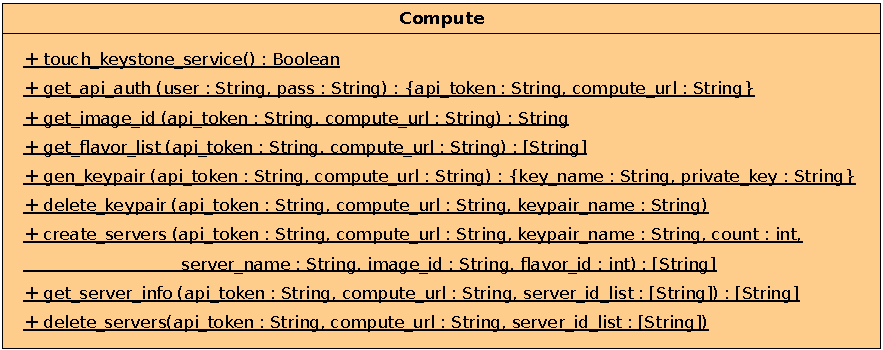
\includegraphics[width=0.99\textwidth]{imagenes/028.pdf}
 \caption{Diagrama de Clases del cliente de acceso REST (II)}
\label{fig:diagramaclasescompute2}
\end{center}
\end{figure}

\begin{description}
 \item[Lista:] \texttt{[TipoDeTodosLosValores]}
 \item[Diccionario:] \texttt{\{<Clave1> : <TipoValor1> ,<Clave2> : <TipoValor2>\}}
\end{description}


\subsubsection{Diagrama de Clases --- Django y Fabric}\label{subsubsec:clasesdjangofabric}
\noindent La figura \ref{fig:djangoyfabric} expone las relaciones entre los m\'odulos m\'as importantes de Django y Fabric. Veamos algunos comentarios sobre el diagrama.

\begin{figure}[tbp]
\begin{center}
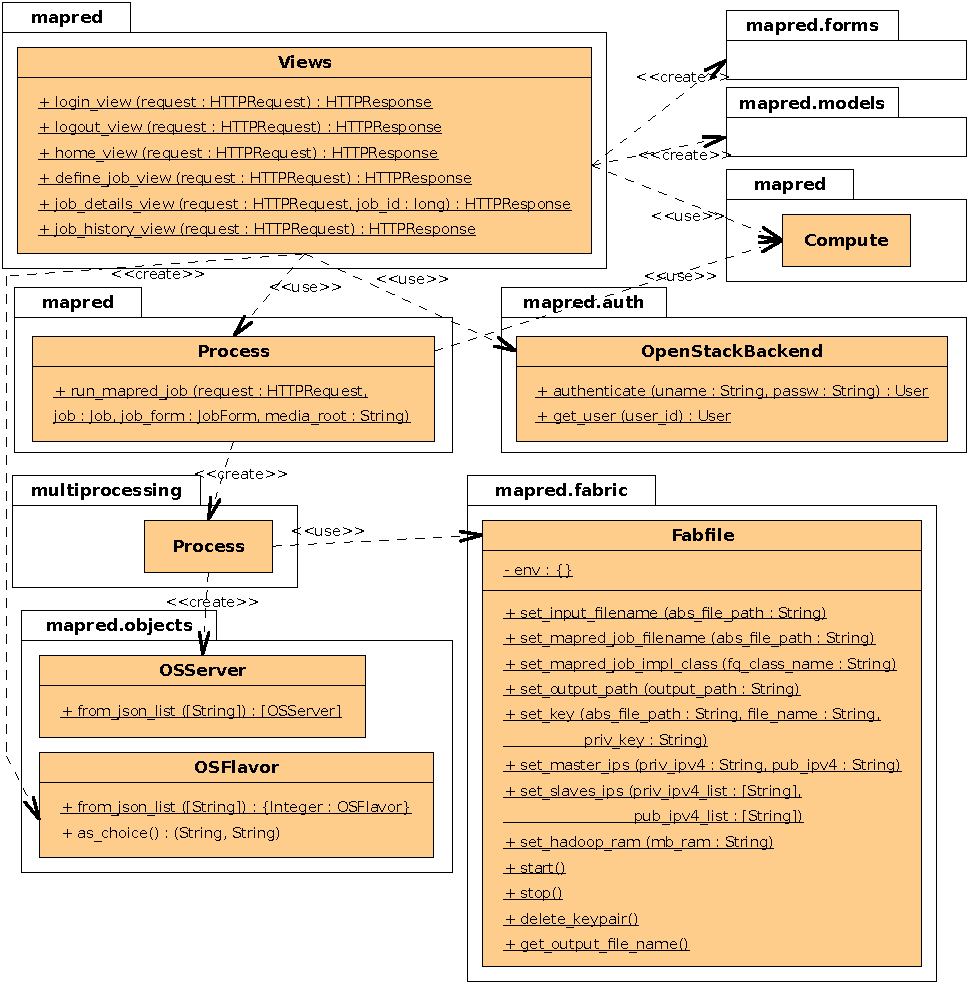
\includegraphics[width=0.99\textwidth]{imagenes/029.pdf}
 \caption{Diagrama de Clases --- Django y Fabric}
\label{fig:djangoyfabric}
\end{center}
\end{figure}

\begin{description}
 \item[Views:] es una clase Django que implementa el comportamiento de cada \emph{vista} (p\'agina web) de la interfaz del proyecto. Interact\'ua directamente con \texttt{Compute} para manejar la comunicaci\'on con el cloud.
 \item[Process:] es una clase wrapper que encapsula tanto el comportamiento de creaci\'on de un proceso \texttt{multiprocessing.Process} como la funci\'on que ejecutar\'a el proceso creado. Esta funci\'on de \texttt{mapred.Process}, cuya firma no se ha incluido por simplicidad, controla el procesado de las instancias Hadoop a trav\'es de \texttt{Compute} y \texttt{Fabfile} (Fabric).
 \item[OpenStackBackend:] es un peque\~no backend que gestiona la conexi\'on de los usuarios. Django incluye un sistema bastante completo para manejar las credenciales de conexi\'on, pero en este proyecto hemos decidido apoyarnos en el de OpenStack para evitar la duplicidad de los usuarios, sus contrase\~nas y datos del perfil. Por tanto, el papel de este backend es hacer de \emph{puente} entre el sistema integrado de credenciales de Django y el de OpenStack; cada petici\'on de conexi\'on se reenv\'ia al \emph{pipe} de acceso a OpenStack. Es decir, s\'olo es necesario que el usuario est\'e registrado en el cloud soporte, OpenStack en nuestro caso, para lanzar trabajos MapReduce.
 \item[OSServer y OSFlavor:] son clases \emph{helper} que desacoplan a la interfaz del servicio REST. Crean representaciones equivalentes en forma de objetos de los JSON que procesan como resultado de las invocaciones de \texttt{Compute}.
\end{description}



\subsubsection{Diagrama de Clases --- Objetos de Django}\label{subsubsec:clasesobjetosdjango}
\noindent La figura \ref{fig:clasesobjetosdjango} contiene, en detalle, las relaciones entre las \emph{clases de objetos del modelo concreto} de Django.


\begin{figure}[tbp]
\begin{center}
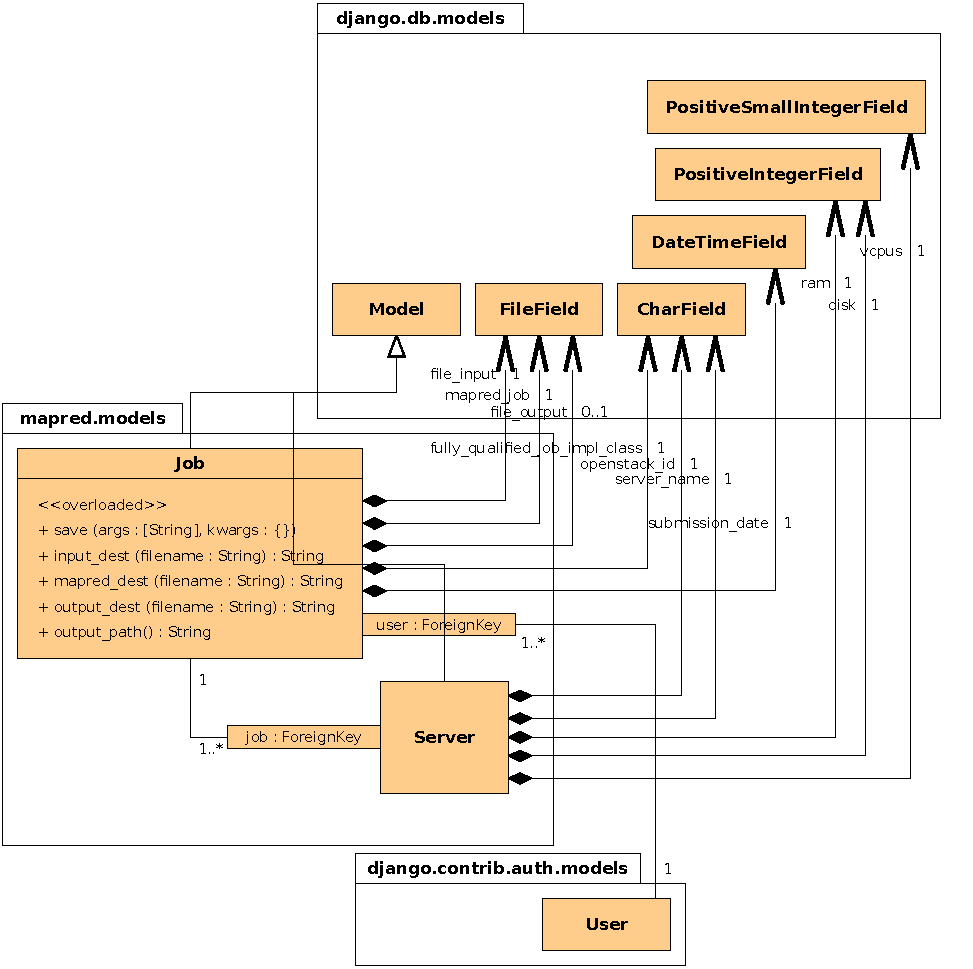
\includegraphics[width=0.99\textwidth]{imagenes/030.pdf}
 \caption{Diagrama de Clases --- Objetos de Django}
\label{fig:clasesobjetosdjango}
\end{center}
\end{figure}


\begin{description}
 \item[django.db.models:] este paquete lo proporciona la distribuci\'on de Django. Sirve de apoyo para escribir objetos del modelo de aplicaci\'on, basados en composiciones y extensiones de las clases contenidas.
  \begin{description}
   \item[Model:] es la clase base de los objetos del modelo, esto es, todo objeto de nuestro minimundo ha de ser \emph{descendiente} suyo. Usando esta clase y las definiciones de las clases de objetos, Django se encargar\'a de gestionar todo lo relativo a la persistencia de los objetos del modelo en una base de datos.
   \item[Fields:] son algunas de las implementaciones m\'as usuales de campos de inter\'es para los objetos que, junto con \texttt{Model}, permiten que Django establezca la morfolog\'ia del esquema l\'ogico de la base de datos asociada.
  \end{description}
 \item[Job:] representa un trabajo MapReduce para Hadoop. Comentar que se ha especializado la definici\'on del m\'etodo \texttt{save}, para poder organizar los trabajos en el sistema de ficheros por su identificador en la base de datos. Tal y como se ha comentado, la salvaguarda de informaci\'on de cada \texttt{Job} en una base datos corre a cargo de Django.
 \item[Server:] es la representaci\'on de la configuraci\'on individual de cada m\'aquina virtual que participe en un trabajo Hadoop MapReduce.
 \item[User:] es la clase interna de Django que almacena la informaci\'on de los usuarios de la interfaz. Se utiliza como \emph{Transfer Object} desde el sistema de autorizaci\'on de OpenStack como portador de los datos de los usuarios en cada \emph{sesi\'on}.
\end{description}


\subsubsection{Diagrama de Clases --- Formularios de Django}\label{subsubsec:clasesformulariosdjango}
\noindent La figura \ref{fig:clasesformulariosdjango} muestra la descomposici\'on en clases de los formularios que recogen las credenciales de acceso y la configuraci\'on del procesado. El paquete \texttt{django.forms} tiene organizaci\'on y finalidad id\'enticos al paquete \texttt{django.db.\\models} comentado anteriormente. En este caso \texttt{Form}, junto con los \texttt{Field} necesarios, es la clase extensible que aporta Django para concretar los formularios de usuario.

\begin{figure}[tbp]
\begin{center}
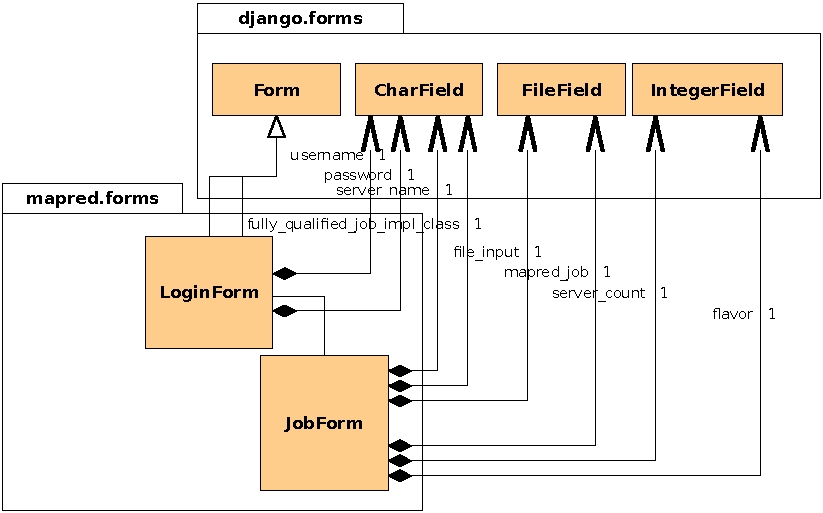
\includegraphics[width=0.99\textwidth]{imagenes/031.pdf}
 \caption{Diagrama de Clases --- Formularios de Django}
\label{fig:clasesformulariosdjango}
\end{center}
\end{figure}

\begin{description}
 \item[LoginForm:] formulario de conexi\'on de usuarios. Formado por un par de campos car\'acter que recogen el nombre de usuario y su contrase\~na en OpenStack.
 \item[JobForm:] es el formulario que permite definir la computaci\'on para \\MapReduce. Incluye: el prefijo del nombre de los servidores virtuales que se crear\'an, el nombre cualificado de la clase implementaci\'on de las funciones Map y Reduce, el fichero de entrada (paquete comprimido), el paquete \emph{Jar} que contiene la clase implementaci\'on, el n\'umero de servidores virtuales necesarios y su \emph{flavor} computacional.
\end{description}


\subsubsection{Diagrama Entidad-Relaci\'on}\label{subsubsec:entidadrelacion}
\noindent Se hab\'ia apuntado brevemente que Django posee la habilidad de construir autom\'aticamente el esquema l\'ogico de una base de datos relacional derivando el modelo de objetos escrito por el desarrollador. Era de esperar que la gesti\'on de las operaciones \emph{CRUD} (\emph{Create, Read, Update, Delete}) sobre las tuplas almacenadas tambi\'en estuviese implementada. La figura \ref{fig:entidadrelacion} muestra el diagrama Entidad-Relaci\'on correspondiente a la gesti\'on de trabajos. Se han omitido las entidades y relaciones adyacentes que gestionan las sesiones o las autorizaciones de los usuarios, entre otras, por transparencia.

\begin{figure}[tbp]
\begin{center}
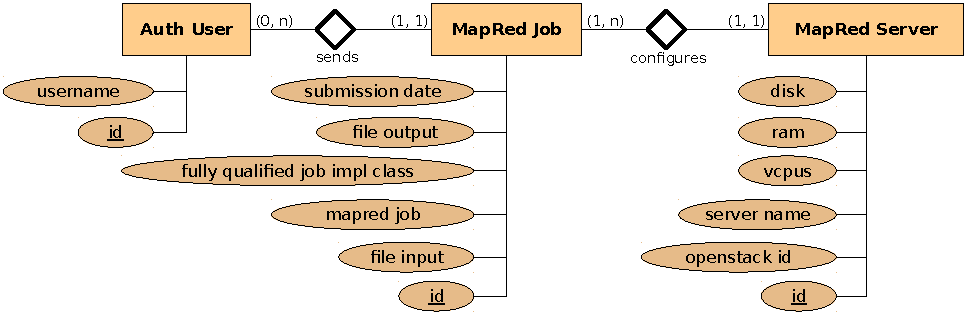
\includegraphics[width=0.99\textwidth]{imagenes/032.pdf}
 \caption{Diagrama Entidad-Relaci\'on}
\label{fig:entidadrelacion}
\end{center}
\end{figure}


\subsubsection{Diagrama de Secuencia}\label{subsubsec:secuencia}

\noindent Se presentan en las figuras \ref{fig:secuencia1} y \ref{fig:secuencia2} dos Diagramas de Secuencia. Reflejan el subconjunto m\'as interesante de los mensajes intercambiados entre las entidades participantes en un procesado MapReduce. Estamos suponiendo que no se produce ning\'un error, que el usuario est\'a conectado a la interfaz con sus credenciales, que introduce correctamente todos los datos de definici\'on del procesado y que posee la autorizaci\'on necesaria para lanzar m\'aquinas virtuales en OpenStack. La figura \ref{fig:secuencia1} contiene la interacci\'on completa. La \ref{fig:secuencia2} expone con detalle la activaci\'on posterior al mensaje \texttt{\#24} de la figura \ref{fig:secuencia1}.

\begin{figure}[tbp]
\begin{center}
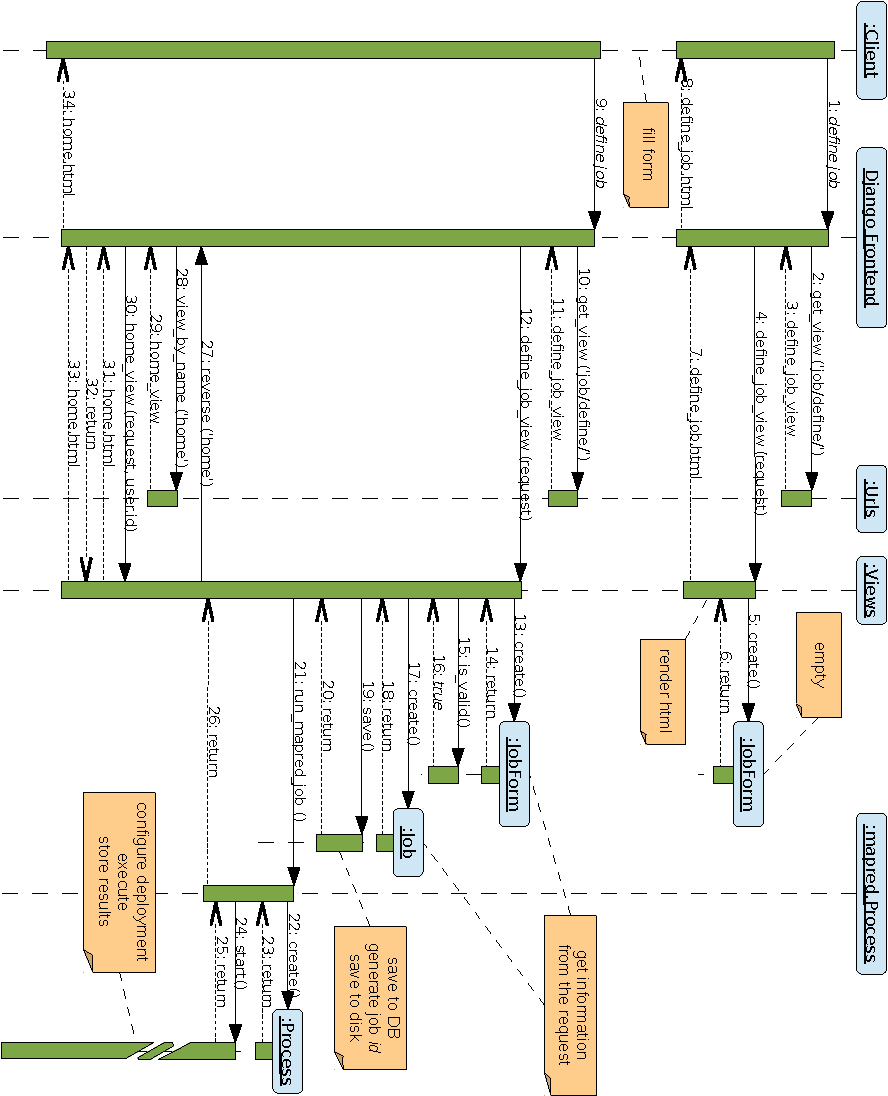
\includegraphics[width=0.99\textwidth]{imagenes/033.pdf}
 \caption{Diagrama de Secuencia (I)}
\label{fig:secuencia1}
\end{center}
\end{figure}

\begin{figure}[tbp]
\begin{center}
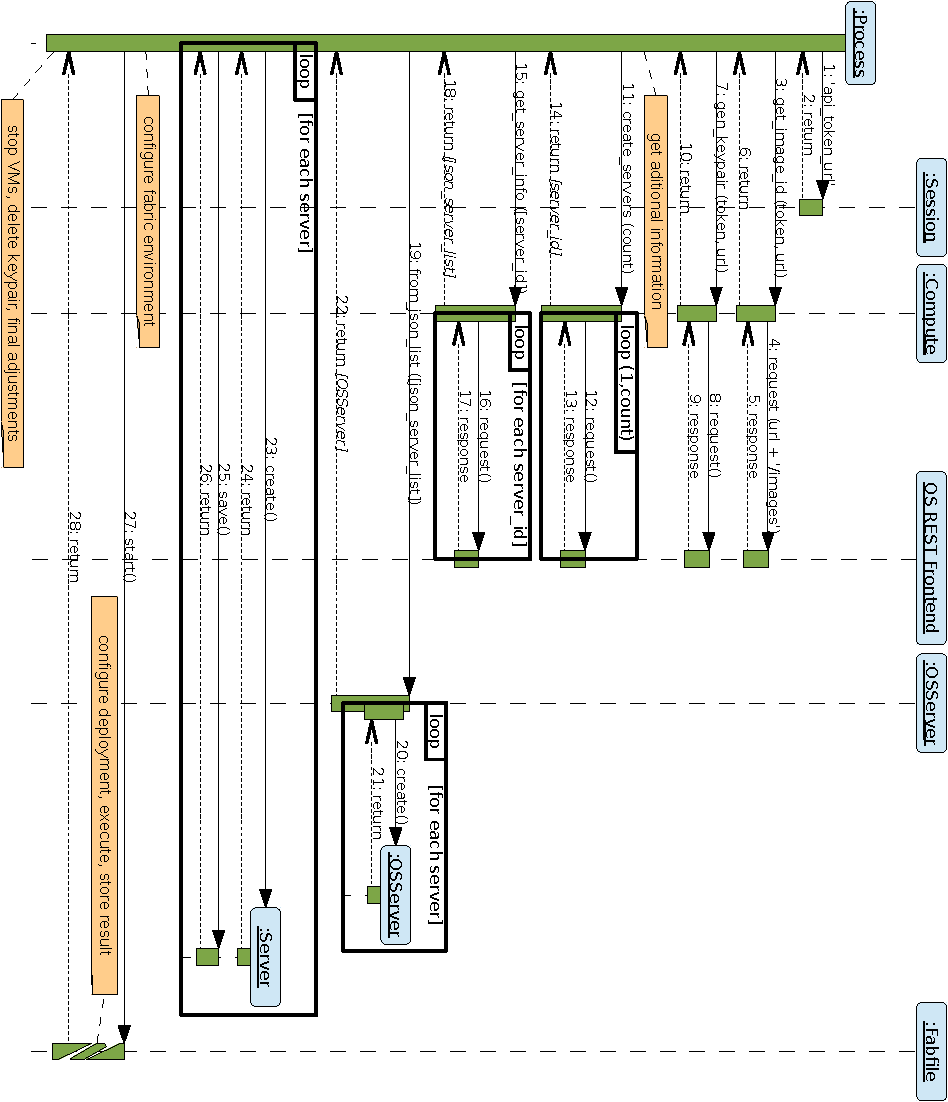
\includegraphics[width=0.99\textwidth]{imagenes/034.pdf}
 \caption{Diagrama de Secuencia (II)}
\label{fig:secuencia2}
\end{center}
\end{figure}

